% This must be in the first 5 lines to tell arXiv to use pdfLaTeX, which is strongly recommended.
% \pdfoutput=1
% In particular, the hyperref package requires pdfLaTeX in order to break URLs across lines.

\documentclass[11pt]{article}

% Change "review" to "final" to generate the final (sometimes called camera-ready) version.
% Change to "preprint" to generate a non-anonymous version with page numbers.
\usepackage{acl}

% Standard package includes
\usepackage{times}
\usepackage{latexsym}

% For proper rendering and hyphenation of words containing Latin characters (including in bib files)
\usepackage[T1]{fontenc}
% For Vietnamese characters
% \usepackage[T5]{fontenc}
% See https://www.latex-project.org/help/documentation/encguide.pdf for other character sets

% This assumes your files are encoded as UTF8
\usepackage[utf8]{inputenc}

% This is not strictly necessary, and may be commented out,
% but it will improve the layout of the manuscript,
% and will typically save some space.
\usepackage{microtype}

% This is also not strictly necessary, and may be commented out.
% However, it will improve the aesthetics of text in
% the typewriter font.
\usepackage{inconsolata}

%Including images in your LaTeX document requires adding
%additional package(s)
\usepackage{graphicx}
\usepackage{booktabs}
\usepackage{float}
\usepackage{amsmath}
\usepackage{soul} % For text highlighting and underlining
\newcommand{\colorul}[2]{\setulcolor{#1}\ul{#2}}
\setul{1.5pt}{0.3ex} % Adjust thickness (1.5pt) and offset (0.3ex)

\definecolor{female}{RGB}{132,33,244}
\definecolor{male}{RGB}{237,117,46}
\definecolor{agricultural}{RGB}{54,33,95}
\definecolor{manufacturing}{RGB}{71,97,214}
\definecolor{construction}{RGB}{44,183,240}
\definecolor{sciences}{RGB}{27,228,183}
\definecolor{logistics}{RGB}{50,242,152}
\definecolor{security}{RGB}{92,252,111}
\definecolor{cleaning}{RGB}{114,254,95}
\definecolor{tourism}{RGB}{156,255,64}
\definecolor{trade}{RGB}{136,255,79}
\definecolor{management}{RGB}{186,246,53}
\definecolor{office}{RGB}{200,239,53}
\definecolor{HR}{RGB}{213,231,54}
\definecolor{finance}{RGB}{235,209,59}
\definecolor{law}{RGB}{244,199,58}
\definecolor{healthcare}{RGB}{253,141,39}
\definecolor{education}{RGB}{202,42,4}
\definecolor{social_work}{RGB}{188,32,2}
\definecolor{design}{RGB}{140,12,5}
\definecolor{journalism}{RGB}{158,17,1}
\definecolor{media}{RGB}{121,4,4}

\usepackage{tikz}
\usetikzlibrary{shapes.geometric, arrows,decorations.pathreplacing}
\tikzstyle{approach} = [rectangle,text width=2.5cm, minimum height=2.5cm, text centered, draw=black, thick]
\tikzstyle{arrow} = [thick,-]
\tikzstyle{start} = [rectangle,text width=4cm, minimum height=1cm, text centered, draw=black, thick]
\tikzstyle{small} = [rectangle,text width=2.5cm, minimum height=1.5cm, text centered, draw=black, thick]
\tikzstyle{smaller} = [rectangle,text width=2cm, minimum height=1.5cm, text centered, draw=black, thick]
\tikzstyle{big} = [rectangle,text width=4cm, minimum height=1.5cm, text centered, draw=black, thick]
\tikzstyle{nope} = [rectangle, text width=2.5cm, minimum height=1.5cm, text centered, draw=white, thick]
\tikzstyle{word} = [rectangle, text width=4cm, minimum height=1cm, draw=white, thick]
\tikzstyle{sentence} = [rectangle, text width=10cm, minimum height=1cm, draw=white, thick]
\tikzstyle{ngram} = [rectangle, text width=2.9cm, minimum height=0.5cm, draw=black, thick]
\tikzstyle{ngram1} = [rectangle, text width=5.5cm, minimum height=0.5cm, draw=black, thick]
\tikzstyle{word2} = [rectangle, minimum height=1cm, draw=white, thick]
\tikzstyle{sen} = [rectangle, minimum height=1cm, draw=white, thick]

% If the title and author information does not fit in the area allocated, uncomment the following
%
%\setlength\titlebox{<dim>}
%
% and set <dim> to something 5cm or larger.

\title{Are All Spanish Doctors Male? \\Evaluating Gender Bias in German Machine Translation}

% Author information can be set in various styles:
% For several authors from the same institution:
% \author{Author 1 \and ... \and Author n \\
%         Address line \\ ... \\ Address line}
% if the names do not fit well on one line use
%         Author 1 \\ {\bf Author 2} \\ ... \\ {\bf Author n} \\
% For authors from different institutions:
% \author{Author 1 \\ Address line \\  ... \\ Address line
%         \And  ... \And
%         Author n \\ Address line \\ ... \\ Address line}
% To start a separate ``row'' of authors use \AND, as in
% \author{Author 1 \\ Address line \\  ... \\ Address line
%         \AND
%         Author 2 \\ Address line \\ ... \\ Address line \And
%         Author 3 \\ Address line \\ ... \\ Address line}

\author{Michelle Kappl \\
  Technische Universität Berlin\\
  \texttt{michelle.kappl@tu-berlin.de}}

%\author{
%  \textbf{First Author\textsuperscript{1}},
%  \textbf{Second Author\textsuperscript{1,2}},
%  \textbf{Third T. Author\textsuperscript{1}},
%  \textbf{Fourth Author\textsuperscript{1}},
%\\
%  \textbf{Fifth Author\textsuperscript{1,2}},
%  \textbf{Sixth Author\textsuperscript{1}},
%  \textbf{Seventh Author\textsuperscript{1}},
%  \textbf{Eighth Author \textsuperscript{1,2,3,4}},
%\\
%  \textbf{Ninth Author\textsuperscript{1}},
%  \textbf{Tenth Author\textsuperscript{1}},
%  \textbf{Eleventh E. Author\textsuperscript{1,2,3,4,5}},
%  \textbf{Twelfth Author\textsuperscript{1}},
%\\
%  \textbf{Thirteenth Author\textsuperscript{3}},
%  \textbf{Fourteenth F. Author\textsuperscript{2,4}},
%  \textbf{Fifteenth Author\textsuperscript{1}},
%  \textbf{Sixteenth Author\textsuperscript{1}},
%\\
%  \textbf{Seventeenth S. Author\textsuperscript{4,5}},
%  \textbf{Eighteenth Author\textsuperscript{3,4}},
%  \textbf{Nineteenth N. Author\textsuperscript{2,5}},
%  \textbf{Twentieth Author\textsuperscript{1}}
%\\
%\\
%  \textsuperscript{1}Affiliation 1,
%  \textsuperscript{2}Affiliation 2,
%  \textsuperscript{3}Affiliation 3,
%  \textsuperscript{4}Affiliation 4,
%  \textsuperscript{5}Affiliation 5
%\\
%  \small{
%    \textbf{Correspondence:} \href{mailto:email@domain}{email@domain}
%  }
%}

\begin{document}
\maketitle
\begin{abstract}

We present WinoMTDE, a new gender bias evaluation test set designed to assess occupational stereotyping and underrepresentation in German machine translation (MT) systems. Building on the automatic evaluation method introduced by \citet{stanovsky-etal-2019-evaluating}, we extend the approach to German, a language with grammatical gender. The WinoMTDE dataset comprises 288 German sentences that are balanced in regard to gender, as well as stereotype, which was annotated using German labor statistics. We conduct a large-scale evaluation of five widely used MT systems and a large language model. Our results reveal persistent bias in most models, with the LLM outperforming traditional systems. The dataset and evaluation code are publicly available at \url{https://github.com/michellekappl/mt_gender_german}.

\end{abstract}

\section{Introduction}

In a globalized world, millions rely on machine translation (MT) systems to break language barriers in medicine, business, and diplomacy every day \citep{vieira_understanding_2021}. However, when these systems fail, the consequences can be severe \citep{Canfora_Ottmann_2020}. The results of a study conducted by \citet{patil_use_2014} show Google
Translate incorrectly translating the phrase \textit{``Your child is fitting''} (which denotes a child
having seizures) into the Swahili equivalent of \textit{``Your child is dead''}. While translation errors in medical contexts can lead to life-threatening misunderstandings, it is not the only domain where MT systems can fail. Another example is depicted in Figure~\ref{fig:gender_bias_example}, where Google Translate mistranslates a sentence from German to Spanish.

\begin{figure}[h]
  \centering
  \resizebox{\columnwidth}{!}{%
  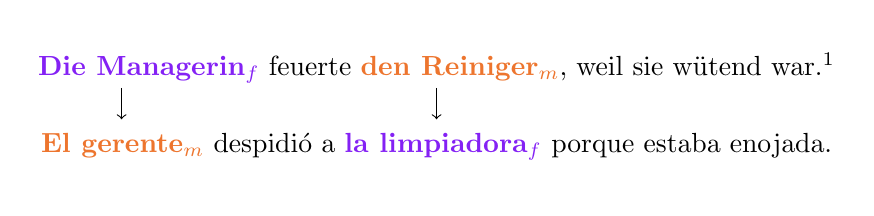
\begin{tikzpicture}
      \node (sen) [sen] {\textbf{\textcolor{female}{Die Managerin$_f$}} feuerte \textbf{\textcolor{male}{den Reiniger$_m$}}, weil sie wütend war.\footnotemark};
      \node (trans) [sen, below of = sen, yshift = 0cm] {\textbf{\textcolor{male}{El gerente$_m$}} despidió a \textbf{\textcolor{female}{la limpiadora$_f$}} porque estaba enojada.};
      \begin{scope}[transform canvas={xshift=0cm}]
          \draw [->] (0,-0.25) -- ++(0,-0.4cm);
      \end{scope}
      \begin{scope}[transform canvas={xshift=-4cm}]
          \draw [->] (0,-0.25) -- ++(0,-0.4cm);
      \end{scope}
  \end{tikzpicture}}
  \caption{Example of gender bias in German Machine Translation by Google Translate, where occupational stereotypes are reinforced.}
  \label{fig:gender_bias_example}
\end{figure}
\footnotetext{Translation: The manager$_f$ fired the cleaner$_m$, because she was mad.}

In this case, the German noun \textit{Die Managerin}, explicitly marked as female, was mistranslated into the masculine Spanish term \textit{El gerente}. Despite clear grammatical markers indicating the subject's gender, the MT system defaulted to a male translation, thereby producing a flawed translation. These phenomena are referred to as gender bias in MT and of rising concern in the field of natural language processing \citep{savoldi_gender_2021,costa-jussa_analysis_2019,blodgett-etal-2020-language}.

\paragraph{Bias Statement \citep{blodgett-etal-2020-language}.}
Gender-biased translations reinforce societal assumptions about the roles and abilities of different genders \citep{vervecken_yes_2015,sterling_confidence_2020}. If MT models systematically misrepresent female subjects and reinforce stereotypical gender roles in occupational contexts, they contribute to the invisibility of women in professions traditionally dominated by men \citep{horvath_does_2016}. Research has shown that children are particularly susceptible to such biases, which can shape their perceptions of career difficulty, prestige, and self-efficacy \citep{vervecken_yes_2015}. Furthermore, \citet{vervecken_yes_2015} found that using pair-forms (e.g., \textit{``Feuerwehrmänner und Feuerwehrfrauen''} for male and female firefighters) instead of male generics increases children's confidence in pursuing non-traditional careers. Studies also highlight a correlation between women's self-efficacy in STEM (Science, Technology, Engineering, and Mathematics) occupations and the persistent gender pay gap \citep{sterling_confidence_2020}.
\paragraph{Contribution.}
To address these issues and minimize potential harm, it is crucial to deepen our understanding of gender bias in MT. Prior research has primarily focused on English MT models, with \citet{stanovsky-etal-2019-evaluating} conducting the first large-scale evaluation on this topic. This work aims to bridge existing research gaps by introducing a German gender bias evaluation testset (GBET), WinoMTDE, which extends the proposed automatic evaluation method developed by \citet{stanovsky-etal-2019-evaluating} to German. The dataset is designed to evaluate occupational stereotyping and gender bias in German MT and therefore enabled us to do a systematic analysis of five widely used MT systems namely Google Translate, Microsoft Translator, Amazon Translate, DeepL, and SYSTRAN. In addition to these traditional MT systems, we also assess GPT-4o-mini, as large language models are increasingly integrated into everyday applications and frequently used for translation tasks \citep{Chan_Tang_2024}. These models were evaluated on their ability to correctly translate sentences from German to seven target languages that heavily exhibit gender in their grammatical structure: French, Italian, Spanish, Ukrainian, Russian, Arabic, and Hebrew. Unlike English, German uses explicit grammatical gender markers, which should, in theory, reduce ambiguity when translating into other gendered languages. One might expect MT systems to produce more accurate and gender-consistent translations due to these grammatical cues. However, despite the availability of such markers, our findings reveal that gender bias persists in most models. This indicates that the problem stems from systemic biases within model architectures and training data rather than source-language ambiguity.
\paragraph{Related Work.}
\citet{stanovsky-etal-2019-evaluating} conducted the first large-scale evaluation of gender bias in English MT systems. They introduced the \textit{WinoMT} GBET, which is based on two corpora of sentences following the Winograd schema \citep{levesque_winograd_2012}, namely \textit{Winogender} \citep{rudinger_gender_2018} and \textit{WinoBias} \citep{zhao_gender_2018}. In their evaluation, they found that all tested MT systems exhibited significant stereotypical and gender bias.

\section{Methodology}
In this section we introduce the WinoMTDE dataset, discuss the evaluation pipeline, and outline the used metrics.

\subsection{WinoMTDE}
We introduce the WinoMTDE\footnote{available at \url{https://github.com/michellekappl/mt_gender_german}} dataset, a German GBET which is a translated subset of WinoMT by \citet{stanovsky-etal-2019-evaluating}. The dataset consists of 288 German sentences structured according to the Winograd schema (see Figure \ref{fig:gender_bias_example}), where each sentence consists of a clearly gendered subject of interest (e.g. \textit{Die Managerin}) in the main clause, as well as another subject of opposite gender (e.g. \textit{der Reiniger}). A pronoun (e.g., \textit{sie}) in a dependent clause refers to the subject of interest. WinoMTDE currently includes only binary-gendered terms and pronouns. It does not account for non-binary pronouns or neutral occupational terms. Each sentence is annotated with:
\begin{itemize}
  \item The subject's \textbf{gender} (male or female).
  \item Its \textbf{position} in the sentence.
  \item The \textbf{stereotype alignment}, i.e. if the occupation is pro- or anti-stereotypical.
\end{itemize}
The dataset is balanced in regard to gender, containing an equal number of female and male-gendered subjects of interest (144 each). \citet{stanovsky-etal-2019-evaluating} used statistics from the U.S. Department of Labor to split WinoMT into equal parts pro- and anti-stereotypical instances. This is used for further evaluating each MT model regarding stereotypical
gender bias. For the WinoMTDE testset to better reflect the German society, statistics from the German Department of Labor (Bundesagentur für Arbeit) were used. Each occupation of the WinoMTDE set was classified according to the \textit{``German Classifications of Occupations 2010 - Revised Version 2020''} \citep{statistik_der_bundesagentur_fur_arbeit_klassifikation_2020}. This classification can be found in the appendix (see \ref{app:occupation_statistics}). By considering the gender distribution of each classified occupation, the stereotypical
gender (defined as more than 50\%) associated with each occupation was determined. For example, the female occupation \textit{Managerin} falls under the category
\textit{``711 - Geschäftsführung und Vorstand''} (managing and board members). Given that 77\% of individuals working in this field are male, the sentence containing \textit{Managerin} is classified as anti-stereotypical.
These subsets, called WinoMTDE$_{anti}$ and WinoMTDE$_{pro}$, contain 121 instances each, therefore making WinoMTDE balanced in regard to stereotype as well. The reduction in size stems from nouns that can not be classified, such as \textit{PatientIn} (patient) or \textit{BesucherIn} (visitor).
\subsection{Evaluation Pipeline}
  \begin{figure}[h]
      \centering
      \includegraphics[width=\columnwidth, height=0.2\textheight]{pipeline.png}
      \caption[Evaluation Pipeline]{Evaluation pipeline \citep{citekey}. The German ground truth is indicated by \textcolor{male}{orange} and the translation by the MT model and the corresponding gender and subject predictions are indicated by \textcolor{female}{violet}.}
      \label{fig:pipeline}
  \end{figure}

  The evaluation pipeline (Figure \ref{fig:pipeline}) based on the work of \citet{stanovsky-etal-2019-evaluating} evaluates translations from German into seven target languages, discussed in \nameref{par:languages}. The pipeline can be divided into three main steps: \textbf{translation}, \textbf{prediction}, and \textbf{evaluation}.
  \paragraph{Translation.}
  As illustrated in Figure \ref{fig:pipeline}, the pipeline is designed to translate each sentence $S$ from the German WinoMTDE testset into a target language, thus producing a corresponding translation $T$ using a selected MT model $M$.
  \begin{table*}
    \resizebox{\textwidth}{!}{%
    \begin{tabular}{cccccccccccccccccccccccccc}
    \toprule
    \multicolumn{1}{c}{} & \multicolumn{3}{c}{\textbf{Google Translate}} & \multicolumn{1}{c}{} & \multicolumn{3}{c}{\textbf{Microsoft Translator}} & \multicolumn{1}{c}{} & \multicolumn{3}{c}{\textbf{Amazon Translate}} & \multicolumn{1}{c}{} &  \multicolumn{3}{c}{\textbf{SYSTRAN}} & \multicolumn{1}{c}{} &  \multicolumn{3}{c}{\textbf{DeepL}} & \multicolumn{1}{c}{} &  \multicolumn{3}{c}{\textbf{GPT-4o-mini}} \\
  
    \cmidrule(lr){2-4} \cmidrule(lr){6-8} \cmidrule(lr){10-12} \cmidrule(lr){14-16} \cmidrule(lr){18-20} \cmidrule(lr){22-24}
  
    \textbf{Languages} & {\textsc{Acc}} & {$\Delta_G$} & {$\Delta_{S}$} && {\textsc{Acc}} & {$\Delta_G$} & {$\Delta_{S}$} && {\textsc{Acc}} & {$\Delta_G$} & {$\Delta_{S'}$} && {\textsc{Acc}} & {$\Delta_G$} & {$\Delta_{S}$} && {\textsc{Acc}} & {$\Delta_G$} & {$\Delta_{S}$} && {\textsc{Acc}} & {$\Delta_G$} & {$\Delta_{S}$}\\
    \midrule
  
    \textit{DE$\rightarrow$ES} & \underline{66.8} & 11.9 & 15.6 && 62.0 & 16.8 & 11.1 &&  \underline{72.7} & 5.2 & 6.8 && \underline{94.1} & 0.1 & 6.6 && 83.1 & 6.4 & 5.6 && \textbf{\underline{95.8}} & 1.7 & -0.8 \\
    \textit{DE$\rightarrow$FR} & 64.2 & 12.1 & 16.2 && \underline{69.2} & 6.2 & 20.9 && 68.0 & 5.7 & 24.5 && 80.6 & 1.5 & -2.7 && \underline{83.3} & 0.4 & -2.3 && \textbf{89.4} & 0.8 & 1.3 \\
    \textit{DE$\rightarrow$IT} & 52.0 & 26.2 & 14.2 && 51.8 & 31.8 & 14.4 && 58.9 & 16.8 & 13.2 && 70.9 & 7.7 & 6.0 && 61.9 & 15.8 & 13.7 && \textbf{75.5 }& 4.4 & 2.3 \\
    \midrule
    \textit{DE$\rightarrow$UK} & 46.5 & 14.7 & 11.6 && 48.2 & 18.8 & 4.0 && 41.4 & 27.4 & 8.0 && 38.2 & 27.4 & -8.2 && 54.7 & 8.2 & 11.7 && \textbf{69.6} & 6.1 & -2.4 \\
    \textit{DE$\rightarrow$RU} & 42.7 & 19.4 & 6.4 && 46.4 & 15.6 & 8.2 && 47.3 & 15.6 & 8.2 && 37.0 & 22.5 & 6.9 && 42.3 & 15.5 & -3.0 && \textbf{55.4} & 6.3 & -15.5 \\
    \midrule
    \textit{DE$\rightarrow$AR} & 55.2 & 18.3 & 9.0 && 54.0 & 20.8 & 9.2 && 59.2 & 15.3 & 7.5 && 51.5 & 24.3 & 10.9 && - & - & - && \textbf{83.3} & 0.5 & 4.9 \\
    \textit{DE$\rightarrow$HE} & 64.5 & 3.8 & 17.5 && 65.4 & 1.9 & 20.9 && 60.3 & 10.0 & 18.7 && 44.6 & 16.1 & 18.4 && - & - & - && \textbf{78.1} & -1.5 & 5.4 \\
    \bottomrule
    \end{tabular}}
    \caption[Results of this Evaluation]{Results of this evaluation for all language pairs. Languages are grouped into their respective language families: Romance, Slavic, and Semitic. The highest accuracy result for each language pair (row-wise) is highlighted in bold, while the best result for each MT model (column-wise) is underlined. DeepL is unable to translate German to either Arabic or Hebrew, which is why the corresponding cells are left empty.}\label{tab:results}
  \end{table*}
  \paragraph{Prediction.} 
  Using \textit{fast-align} the source and target sentence get mapped to one another. It is a word alignment tool that was developed by \citet{dyer_simple_2013} and produces a word alignment in the "Pharao format". For each word index in $S$ \textit{fast-align} finds the corresponding word index in $T$.  This means that the word, that is our subject of interest in $S$ is aligned with the corresponding word in $T$. Furthermore, especially in the Romance languages, where each noun has a gendered noun determiner, the gender is often clearly encoded in the articles. To improve prediction quality the subject of interest as well as the corresponding article are used for the morphological analysis. Language-specific tools   like \textit{spaCy} (for Romance languages), \textit{pymorphy2} (for Slavic languages), and the morphological analyzer by \citet{adler_unsupervised_2006} (for Hebrew) determine the gender of the nouns. For Arabic, gender is inferred using the ta marbuta character, a marker of femininity. If it is not possible to determine the gender of a word, it is marked as unknown. Furthermore, gender-neutral terms, such as the Spanish word \textit{estudiante} (student, no specified gender) are annotated as neutral.
  Using the predicted gender information on the translated subject of interest different metrics are calculated to evaluate the MT model $M$.
  \paragraph{Evaluation.}
  The evaluation is based on the following metrics.
  \begin{description}
    \item[Accuracy.] For each model $M$ the general accuracy is calculated and denotes the percentage of instances where the ground truth gender (annotated in WinoMTDE) matches the predicted gender. It is calculated as follows:
    \begin{align*}
      \text{\textsc{acc}} = \frac{\text{total number of correct predictions}}{\text{total number of predictions}}
    \end{align*}
    \item[Gender-based F1-score gap $\Delta_G$.] The F1-score is a metric that combines precision and recall. Precision is defined as the ratio between correct predictions and the total number of predictions. Recall on the other hand is the ratio between correct predictions and the total number of instances. Both of these metrics are calculated using the WinoMTDE set as the ground truth and with the following formulas, where the gender $g$ is either male Using this the respective F1-Scores can be calculated as follows:
    \begin{align*}
        \text{\textsc{F1-score}}_g &= 2 \cdot \frac{\text{Precision}_g \cdot \text{Recall}_g}{\text{Precision}_g + \text{Recall}_g}
    \end{align*}
    After calculating both the male and the female \textsc{F1-score}, $\Delta_G$ is defined by following formula:
    \begin{align*}
        \Delta_{G} = \text{\textsc{F1-score}}_m - \text{\textsc{F1-score}}_f
    \end{align*}
    \item[Stereotype-based performance gap $\Delta_{S}$.]
    \citet{stanovsky-etal-2019-evaluating} defines $\Delta_S$ as the "difference in performance (F1-score)\footnote{It is important to note that even though the paper states that it utilizes the F1-score (although no formula is given) the actual calculation within the code published on GitHub is done using Accuracy.} between stereotypical and non-stereotypical gender role assignments". In contrast to the metrics discussed previously, it utilizes the subsets of WinoMTDE that are classified as stereotypical (WinoMTDE$_{pro}$) and anti-stereotypical (WinoMTDE$_{anti}$). $\Delta_S$ is calculated as follows:
    \begin{align*}
        \Delta_{S} = \text{\textsc{Acc}}_{pro} - \text{\textsc{Acc}}_{anti}
    \end{align*}
\end{description}


\section{Experimental Setup}
Using the evaluation pipeline, we evaluate six MT models on seven languages.
\paragraph{MT Models.} The original paper by \citet{stanovsky-etal-2019-evaluating} evaluated five commercial MT systems, namely Google Translate (GT), Microsoft Translator (Micr. T), Amazon Translate (AT), and SYSTRAN (S). In addition to these models, we also evaluate DeepL (D) and GPT-4o-mini (4o-m). The models were selected based on their popularity, availability, and the comparability of the results with the original study. Most of these models are neural machine translation systems, except for SYSTRAN, which is a hybrid system combining rule-based and statistical MT and GPT-4o-mini, a large language model.
\paragraph{Languages.}\label{par:languages} The models are evaluated on their ability to translate German sentences into seven target languages: Hebrew (HE), Arabic (AR), Spanish (ES), French (FR), Italian (IT), Russian (RU), and Ukrainian (UK). These languages were selected based on their gendered grammatical structure and different language families.

\section{Results}
The main results of this evaluation are presented in Table \ref{tab:results}, highlighting the performance of each model across accuracy, gender-based F1-score gaps ($\Delta_G$), and stereotype-based performance gaps ($\Delta_S$). 
\begin{figure*}[h]
  \centering
  \includegraphics[width=\textwidth]{pred_dist.png}
  \caption[Gender Distribution for all Occupation Groups and Models]{Gender predictions for each occupation group across all languages and MT models were aggregated and visualized. Colors represent professional categories: blue hues for \colorul{agricultural}{agricultural}, \colorul{manufacturing}{manufacturing}, and \colorul{construction}{construction}; turquoise for \colorul{sciences}{sciences}, \colorul{logistics}{logistics}, and \colorul{security}{security}; green for \colorul{cleaning}{cleaning}, \colorul{tourism}{tourism}, and \colorul{trade}{trade}; greenish-yellow for \colorul{management}{management}, \colorul{office}{office}, and \colorul{HR}{HR}; yellow for \colorul{finance}{finance} and \colorul{law}{law}; orange for \colorul{healthcare}{healthcare}; red for \colorul{education}{education} and \colorul{social_work}{social work}; and dark red for \colorul{media}{media}, \colorul{journalism}{journalism}, and \colorul{design}{design}. The x-axis corresponds to the real-world distribution of each occupation group (see \ref{app:occupation_statistics}), ranging from 100\% female workers on the left to a 50\% (50\% male) balance in the middle, and finally to 0\% (100\% male) on the right. The grey vertical line marks occupations with minimal gender imbalance in the real world. The y-axis represents the gender distribution within the translated challenge set. An ideal translation would result in all markers aligning with the green horizontal line, indicating preserved original distribution as WinoMTDE is balanced in terms of gender and stereotypes.}
  \label{fig:prediction_dist}
\end{figure*}

The \textbf{accuracy} results, measuring how well a model preserves the original gender, range from 37.0\% to 95.8\%, showing significant performance differences across models and language pairs. GPT-4o-mini consistently achieves the highest accuracy across all language pairs, outperforming other MT systems. SYSTRAN, the only hybrid model evaluated, performs particularly well in the Romance language family, outperforming most neural models. Performance in the Slavic languages is weaker, with only GPT-4o-mini and DeepL surpassing the 50\% accuracy threshold, which indicates a performance better than random guessing. Google Translate performs the weakest overall.\\
The \textbf{gender-based F1-score gap} ($\Delta_G$) measures disparities between translations of male and female instances, with zero being the optimal score. Positive values indicate better performance on male instances, while a negative value reflects better performance on female instances. Across all models, the results reveal a consistent bias, with an average $\Delta_G$ of 11.9\%, indicating that models generally perform better on male instances. GPT-4o-mini stands out with the lowest average (2.4\%) across language pairs, indicating a less gender biased translation. DeepL also shows relatively good performance, even though it is outperformed by SYSTRAN in the Romance language family. \\
The \textbf{stereotype-based performance gap} ($\Delta_S$), which measures differences between stereotypical and anti-stereotypical translations, averages at 8.51\% across all models and languages. The performance gap is most noticeable in Romance languages, where Amazon Translate exhibits the largest $\Delta_S$, showing a strong bias towards non-stereotypical gender roles. Generally, GPT-4o-mini consistently exhibits lower scores than the other models, except for a strong non-stereotypical bias in Russian translations. 

The patterns observed in Table \ref{tab:results} are further illustrated in Figure \ref{fig:prediction_dist}, which visualizes the distribution of gender predictions across different occupational groups and models. While GPT-4o-mini often closely aligns, i.e. is within the green margin, with the perfect translation of the balanced WinoMTDE dataset, other models exhibit patterns that reflect or exaggerate real-world gender imbalances. Generally speaking, the results show that models tend to exhibit a strong bias towards male translations across all occupational groups, as indicated by the majority of markers falling into the upper two quadrants.

Overall, the results demonstrate that GPT-4o-mini achieves the strongest performance across all metrics, with SYSTRAN and DeepL also performing competitively, especially in Romance languages. The findings highlight significant weaknesses in Google Translate, which underperforms despite its widespread use.
\section{Discussion}
Generally, our results find that underrepresentation of females as well as stereotypical bias, although not as pronounced, is prevalent in most MT system. GPT-4o-mini, a large language model, consistently outperforms traditional MT systems, such as Google Translate, Microsoft Translator, Amazon Translate, and DeepL.
Nevertheless, it exhibits bias, particularly in Russian translations. This may stem from OpenAI's use of user data to train its models, but prohibiting Russians access to their models. This could lead to a lack of data and therefore the model might not be able to generalize well to the Russian language.
Furthermore, the results suggest that using hybrid MT models, such as SYSTRAN can lead to better results in Romance languages. This is especially interesting as it indicates that using set grammatical rules could be a possibility to minimize gender bias within MT from German to Romance languages. However,
SYSTRAN performed worse than the other MT models within the Slavic and Semitic language families. This could be due to the fact that the grammatical rules to translate to those languages are more complex and therefore harder to implement.

\subsection{Limitations and Future Work}
Despite providing valuable insights, this evaluation has several limitations. First, the WinoMTDE dataset is relatively small (288 sentences), potentially limiting the scope of gender bias that can be assessed. Stereotype annotations were based on German labor statistics and annotated by a single person, which may introduce bias, especially for ambiguous job titles (e.g., \textit{UntersucherIn}, meaning both ``examiner'' and ``investigator''). Additionally, the broad grouping of occupations fails to capture nuanced stereotypes within fields. The dataset also lacks non-binary pronouns and neutral job titles, restricting the analysis to a binary gender perspective and overlooking broader gender biases. Certain biases, like semantic derogation, are also unaddressed. For example, translating ``teacher'' into Spanish produced gendered terms (\textit{maestra} for female and \textit{profesor} for male subjects), reinforcing stereotypes.

Moreover, this paper reports a higher share of unknown predictions compared to prior work, likely due to challenges with sentence alignment in \textit{fast-align}, particularly with complex German structures. SYSTRAN, a hybrid model, showed fewer unknown predictions, possibly due to its rule-based approach (see Figure \ref{fig:romance}). Thus, the models' actual accuracy might be higher than reported. A table of accuracies excluding unknown predictions is provided in the appendix (see \ref{app:accuracy_wo_unknown}).

\begin{figure}[h]
  \centering
  \includegraphics[width=\columnwidth]{romance.png}
  \caption[Gender Distribution of Translations by GPT-4o-mini, DeepL and SYSTRAN]{Depiction of the percentage of female (violet), male (orange), neutral (blue), and unknown (light blue) translations across occupations. Dark shades represent correct gender matches, light shades indicate errors. Hatching shows the gender origin within neutral and unknown categories. The horizontal line marks the 50/50 male-female ground truth.}
  \label{fig:romance}
\end{figure}

Future work should address these limitations by expanding the dataset, refining stereotype annotations, and including non-binary pronouns and neutral job titles. The evaluation pipeline could also be improved by using more advanced alignment tools to reduce unknown predictions. Additionally, evaluating MT models with known architectures and training data may provide deeper insights into observed biases.
\subsection{Conclusion}
In order to better understand gender bias and its emerging harms,
it is crucial to evaluate MT systems systematically. The WinoMTDE
dataset and evaluation methodology provide the first foundation
for this evaluation in German MT. The results of the evaluation of five MT models and a general-purpose LLM, highlight the persistent gender bias within translations. These results emphasize the urgent need to develop more inclusive and equitable MT systems that ensure both accuracy and fairness in translations.
\newpage \newpage
\bibliography{main}

\appendix
\subsection{Lloyd-Max Algorithm}
\label{subsec:Lloyd-Max}
For a given quantization bitwidth $B$ and an operand $\bm{X}$, the Lloyd-Max algorithm finds $2^B$ quantization levels $\{\hat{x}_i\}_{i=1}^{2^B}$ such that quantizing $\bm{X}$ by rounding each scalar in $\bm{X}$ to the nearest quantization level minimizes the quantization MSE. 

The algorithm starts with an initial guess of quantization levels and then iteratively computes quantization thresholds $\{\tau_i\}_{i=1}^{2^B-1}$ and updates quantization levels $\{\hat{x}_i\}_{i=1}^{2^B}$. Specifically, at iteration $n$, thresholds are set to the midpoints of the previous iteration's levels:
\begin{align*}
    \tau_i^{(n)}=\frac{\hat{x}_i^{(n-1)}+\hat{x}_{i+1}^{(n-1)}}2 \text{ for } i=1\ldots 2^B-1
\end{align*}
Subsequently, the quantization levels are re-computed as conditional means of the data regions defined by the new thresholds:
\begin{align*}
    \hat{x}_i^{(n)}=\mathbb{E}\left[ \bm{X} \big| \bm{X}\in [\tau_{i-1}^{(n)},\tau_i^{(n)}] \right] \text{ for } i=1\ldots 2^B
\end{align*}
where to satisfy boundary conditions we have $\tau_0=-\infty$ and $\tau_{2^B}=\infty$. The algorithm iterates the above steps until convergence.

Figure \ref{fig:lm_quant} compares the quantization levels of a $7$-bit floating point (E3M3) quantizer (left) to a $7$-bit Lloyd-Max quantizer (right) when quantizing a layer of weights from the GPT3-126M model at a per-tensor granularity. As shown, the Lloyd-Max quantizer achieves substantially lower quantization MSE. Further, Table \ref{tab:FP7_vs_LM7} shows the superior perplexity achieved by Lloyd-Max quantizers for bitwidths of $7$, $6$ and $5$. The difference between the quantizers is clear at 5 bits, where per-tensor FP quantization incurs a drastic and unacceptable increase in perplexity, while Lloyd-Max quantization incurs a much smaller increase. Nevertheless, we note that even the optimal Lloyd-Max quantizer incurs a notable ($\sim 1.5$) increase in perplexity due to the coarse granularity of quantization. 

\begin{figure}[h]
  \centering
  \includegraphics[width=0.7\linewidth]{sections/figures/LM7_FP7.pdf}
  \caption{\small Quantization levels and the corresponding quantization MSE of Floating Point (left) vs Lloyd-Max (right) Quantizers for a layer of weights in the GPT3-126M model.}
  \label{fig:lm_quant}
\end{figure}

\begin{table}[h]\scriptsize
\begin{center}
\caption{\label{tab:FP7_vs_LM7} \small Comparing perplexity (lower is better) achieved by floating point quantizers and Lloyd-Max quantizers on a GPT3-126M model for the Wikitext-103 dataset.}
\begin{tabular}{c|cc|c}
\hline
 \multirow{2}{*}{\textbf{Bitwidth}} & \multicolumn{2}{|c|}{\textbf{Floating-Point Quantizer}} & \textbf{Lloyd-Max Quantizer} \\
 & Best Format & Wikitext-103 Perplexity & Wikitext-103 Perplexity \\
\hline
7 & E3M3 & 18.32 & 18.27 \\
6 & E3M2 & 19.07 & 18.51 \\
5 & E4M0 & 43.89 & 19.71 \\
\hline
\end{tabular}
\end{center}
\end{table}

\subsection{Proof of Local Optimality of LO-BCQ}
\label{subsec:lobcq_opt_proof}
For a given block $\bm{b}_j$, the quantization MSE during LO-BCQ can be empirically evaluated as $\frac{1}{L_b}\lVert \bm{b}_j- \bm{\hat{b}}_j\rVert^2_2$ where $\bm{\hat{b}}_j$ is computed from equation (\ref{eq:clustered_quantization_definition}) as $C_{f(\bm{b}_j)}(\bm{b}_j)$. Further, for a given block cluster $\mathcal{B}_i$, we compute the quantization MSE as $\frac{1}{|\mathcal{B}_{i}|}\sum_{\bm{b} \in \mathcal{B}_{i}} \frac{1}{L_b}\lVert \bm{b}- C_i^{(n)}(\bm{b})\rVert^2_2$. Therefore, at the end of iteration $n$, we evaluate the overall quantization MSE $J^{(n)}$ for a given operand $\bm{X}$ composed of $N_c$ block clusters as:
\begin{align*}
    \label{eq:mse_iter_n}
    J^{(n)} = \frac{1}{N_c} \sum_{i=1}^{N_c} \frac{1}{|\mathcal{B}_{i}^{(n)}|}\sum_{\bm{v} \in \mathcal{B}_{i}^{(n)}} \frac{1}{L_b}\lVert \bm{b}- B_i^{(n)}(\bm{b})\rVert^2_2
\end{align*}

At the end of iteration $n$, the codebooks are updated from $\mathcal{C}^{(n-1)}$ to $\mathcal{C}^{(n)}$. However, the mapping of a given vector $\bm{b}_j$ to quantizers $\mathcal{C}^{(n)}$ remains as  $f^{(n)}(\bm{b}_j)$. At the next iteration, during the vector clustering step, $f^{(n+1)}(\bm{b}_j)$ finds new mapping of $\bm{b}_j$ to updated codebooks $\mathcal{C}^{(n)}$ such that the quantization MSE over the candidate codebooks is minimized. Therefore, we obtain the following result for $\bm{b}_j$:
\begin{align*}
\frac{1}{L_b}\lVert \bm{b}_j - C_{f^{(n+1)}(\bm{b}_j)}^{(n)}(\bm{b}_j)\rVert^2_2 \le \frac{1}{L_b}\lVert \bm{b}_j - C_{f^{(n)}(\bm{b}_j)}^{(n)}(\bm{b}_j)\rVert^2_2
\end{align*}

That is, quantizing $\bm{b}_j$ at the end of the block clustering step of iteration $n+1$ results in lower quantization MSE compared to quantizing at the end of iteration $n$. Since this is true for all $\bm{b} \in \bm{X}$, we assert the following:
\begin{equation}
\begin{split}
\label{eq:mse_ineq_1}
    \tilde{J}^{(n+1)} &= \frac{1}{N_c} \sum_{i=1}^{N_c} \frac{1}{|\mathcal{B}_{i}^{(n+1)}|}\sum_{\bm{b} \in \mathcal{B}_{i}^{(n+1)}} \frac{1}{L_b}\lVert \bm{b} - C_i^{(n)}(b)\rVert^2_2 \le J^{(n)}
\end{split}
\end{equation}
where $\tilde{J}^{(n+1)}$ is the the quantization MSE after the vector clustering step at iteration $n+1$.

Next, during the codebook update step (\ref{eq:quantizers_update}) at iteration $n+1$, the per-cluster codebooks $\mathcal{C}^{(n)}$ are updated to $\mathcal{C}^{(n+1)}$ by invoking the Lloyd-Max algorithm \citep{Lloyd}. We know that for any given value distribution, the Lloyd-Max algorithm minimizes the quantization MSE. Therefore, for a given vector cluster $\mathcal{B}_i$ we obtain the following result:

\begin{equation}
    \frac{1}{|\mathcal{B}_{i}^{(n+1)}|}\sum_{\bm{b} \in \mathcal{B}_{i}^{(n+1)}} \frac{1}{L_b}\lVert \bm{b}- C_i^{(n+1)}(\bm{b})\rVert^2_2 \le \frac{1}{|\mathcal{B}_{i}^{(n+1)}|}\sum_{\bm{b} \in \mathcal{B}_{i}^{(n+1)}} \frac{1}{L_b}\lVert \bm{b}- C_i^{(n)}(\bm{b})\rVert^2_2
\end{equation}

The above equation states that quantizing the given block cluster $\mathcal{B}_i$ after updating the associated codebook from $C_i^{(n)}$ to $C_i^{(n+1)}$ results in lower quantization MSE. Since this is true for all the block clusters, we derive the following result: 
\begin{equation}
\begin{split}
\label{eq:mse_ineq_2}
     J^{(n+1)} &= \frac{1}{N_c} \sum_{i=1}^{N_c} \frac{1}{|\mathcal{B}_{i}^{(n+1)}|}\sum_{\bm{b} \in \mathcal{B}_{i}^{(n+1)}} \frac{1}{L_b}\lVert \bm{b}- C_i^{(n+1)}(\bm{b})\rVert^2_2  \le \tilde{J}^{(n+1)}   
\end{split}
\end{equation}

Following (\ref{eq:mse_ineq_1}) and (\ref{eq:mse_ineq_2}), we find that the quantization MSE is non-increasing for each iteration, that is, $J^{(1)} \ge J^{(2)} \ge J^{(3)} \ge \ldots \ge J^{(M)}$ where $M$ is the maximum number of iterations. 
%Therefore, we can say that if the algorithm converges, then it must be that it has converged to a local minimum. 
\hfill $\blacksquare$


\begin{figure}
    \begin{center}
    \includegraphics[width=0.5\textwidth]{sections//figures/mse_vs_iter.pdf}
    \end{center}
    \caption{\small NMSE vs iterations during LO-BCQ compared to other block quantization proposals}
    \label{fig:nmse_vs_iter}
\end{figure}

Figure \ref{fig:nmse_vs_iter} shows the empirical convergence of LO-BCQ across several block lengths and number of codebooks. Also, the MSE achieved by LO-BCQ is compared to baselines such as MXFP and VSQ. As shown, LO-BCQ converges to a lower MSE than the baselines. Further, we achieve better convergence for larger number of codebooks ($N_c$) and for a smaller block length ($L_b$), both of which increase the bitwidth of BCQ (see Eq \ref{eq:bitwidth_bcq}).


\subsection{Additional Accuracy Results}
%Table \ref{tab:lobcq_config} lists the various LOBCQ configurations and their corresponding bitwidths.
\begin{table}
\setlength{\tabcolsep}{4.75pt}
\begin{center}
\caption{\label{tab:lobcq_config} Various LO-BCQ configurations and their bitwidths.}
\begin{tabular}{|c||c|c|c|c||c|c||c|} 
\hline
 & \multicolumn{4}{|c||}{$L_b=8$} & \multicolumn{2}{|c||}{$L_b=4$} & $L_b=2$ \\
 \hline
 \backslashbox{$L_A$\kern-1em}{\kern-1em$N_c$} & 2 & 4 & 8 & 16 & 2 & 4 & 2 \\
 \hline
 64 & 4.25 & 4.375 & 4.5 & 4.625 & 4.375 & 4.625 & 4.625\\
 \hline
 32 & 4.375 & 4.5 & 4.625& 4.75 & 4.5 & 4.75 & 4.75 \\
 \hline
 16 & 4.625 & 4.75& 4.875 & 5 & 4.75 & 5 & 5 \\
 \hline
\end{tabular}
\end{center}
\end{table}

%\subsection{Perplexity achieved by various LO-BCQ configurations on Wikitext-103 dataset}

\begin{table} \centering
\begin{tabular}{|c||c|c|c|c||c|c||c|} 
\hline
 $L_b \rightarrow$& \multicolumn{4}{c||}{8} & \multicolumn{2}{c||}{4} & 2\\
 \hline
 \backslashbox{$L_A$\kern-1em}{\kern-1em$N_c$} & 2 & 4 & 8 & 16 & 2 & 4 & 2  \\
 %$N_c \rightarrow$ & 2 & 4 & 8 & 16 & 2 & 4 & 2 \\
 \hline
 \hline
 \multicolumn{8}{c}{GPT3-1.3B (FP32 PPL = 9.98)} \\ 
 \hline
 \hline
 64 & 10.40 & 10.23 & 10.17 & 10.15 &  10.28 & 10.18 & 10.19 \\
 \hline
 32 & 10.25 & 10.20 & 10.15 & 10.12 &  10.23 & 10.17 & 10.17 \\
 \hline
 16 & 10.22 & 10.16 & 10.10 & 10.09 &  10.21 & 10.14 & 10.16 \\
 \hline
  \hline
 \multicolumn{8}{c}{GPT3-8B (FP32 PPL = 7.38)} \\ 
 \hline
 \hline
 64 & 7.61 & 7.52 & 7.48 &  7.47 &  7.55 &  7.49 & 7.50 \\
 \hline
 32 & 7.52 & 7.50 & 7.46 &  7.45 &  7.52 &  7.48 & 7.48  \\
 \hline
 16 & 7.51 & 7.48 & 7.44 &  7.44 &  7.51 &  7.49 & 7.47  \\
 \hline
\end{tabular}
\caption{\label{tab:ppl_gpt3_abalation} Wikitext-103 perplexity across GPT3-1.3B and 8B models.}
\end{table}

\begin{table} \centering
\begin{tabular}{|c||c|c|c|c||} 
\hline
 $L_b \rightarrow$& \multicolumn{4}{c||}{8}\\
 \hline
 \backslashbox{$L_A$\kern-1em}{\kern-1em$N_c$} & 2 & 4 & 8 & 16 \\
 %$N_c \rightarrow$ & 2 & 4 & 8 & 16 & 2 & 4 & 2 \\
 \hline
 \hline
 \multicolumn{5}{|c|}{Llama2-7B (FP32 PPL = 5.06)} \\ 
 \hline
 \hline
 64 & 5.31 & 5.26 & 5.19 & 5.18  \\
 \hline
 32 & 5.23 & 5.25 & 5.18 & 5.15  \\
 \hline
 16 & 5.23 & 5.19 & 5.16 & 5.14  \\
 \hline
 \multicolumn{5}{|c|}{Nemotron4-15B (FP32 PPL = 5.87)} \\ 
 \hline
 \hline
 64  & 6.3 & 6.20 & 6.13 & 6.08  \\
 \hline
 32  & 6.24 & 6.12 & 6.07 & 6.03  \\
 \hline
 16  & 6.12 & 6.14 & 6.04 & 6.02  \\
 \hline
 \multicolumn{5}{|c|}{Nemotron4-340B (FP32 PPL = 3.48)} \\ 
 \hline
 \hline
 64 & 3.67 & 3.62 & 3.60 & 3.59 \\
 \hline
 32 & 3.63 & 3.61 & 3.59 & 3.56 \\
 \hline
 16 & 3.61 & 3.58 & 3.57 & 3.55 \\
 \hline
\end{tabular}
\caption{\label{tab:ppl_llama7B_nemo15B} Wikitext-103 perplexity compared to FP32 baseline in Llama2-7B and Nemotron4-15B, 340B models}
\end{table}

%\subsection{Perplexity achieved by various LO-BCQ configurations on MMLU dataset}


\begin{table} \centering
\begin{tabular}{|c||c|c|c|c||c|c|c|c|} 
\hline
 $L_b \rightarrow$& \multicolumn{4}{c||}{8} & \multicolumn{4}{c||}{8}\\
 \hline
 \backslashbox{$L_A$\kern-1em}{\kern-1em$N_c$} & 2 & 4 & 8 & 16 & 2 & 4 & 8 & 16  \\
 %$N_c \rightarrow$ & 2 & 4 & 8 & 16 & 2 & 4 & 2 \\
 \hline
 \hline
 \multicolumn{5}{|c|}{Llama2-7B (FP32 Accuracy = 45.8\%)} & \multicolumn{4}{|c|}{Llama2-70B (FP32 Accuracy = 69.12\%)} \\ 
 \hline
 \hline
 64 & 43.9 & 43.4 & 43.9 & 44.9 & 68.07 & 68.27 & 68.17 & 68.75 \\
 \hline
 32 & 44.5 & 43.8 & 44.9 & 44.5 & 68.37 & 68.51 & 68.35 & 68.27  \\
 \hline
 16 & 43.9 & 42.7 & 44.9 & 45 & 68.12 & 68.77 & 68.31 & 68.59  \\
 \hline
 \hline
 \multicolumn{5}{|c|}{GPT3-22B (FP32 Accuracy = 38.75\%)} & \multicolumn{4}{|c|}{Nemotron4-15B (FP32 Accuracy = 64.3\%)} \\ 
 \hline
 \hline
 64 & 36.71 & 38.85 & 38.13 & 38.92 & 63.17 & 62.36 & 63.72 & 64.09 \\
 \hline
 32 & 37.95 & 38.69 & 39.45 & 38.34 & 64.05 & 62.30 & 63.8 & 64.33  \\
 \hline
 16 & 38.88 & 38.80 & 38.31 & 38.92 & 63.22 & 63.51 & 63.93 & 64.43  \\
 \hline
\end{tabular}
\caption{\label{tab:mmlu_abalation} Accuracy on MMLU dataset across GPT3-22B, Llama2-7B, 70B and Nemotron4-15B models.}
\end{table}


%\subsection{Perplexity achieved by various LO-BCQ configurations on LM evaluation harness}

\begin{table} \centering
\begin{tabular}{|c||c|c|c|c||c|c|c|c|} 
\hline
 $L_b \rightarrow$& \multicolumn{4}{c||}{8} & \multicolumn{4}{c||}{8}\\
 \hline
 \backslashbox{$L_A$\kern-1em}{\kern-1em$N_c$} & 2 & 4 & 8 & 16 & 2 & 4 & 8 & 16  \\
 %$N_c \rightarrow$ & 2 & 4 & 8 & 16 & 2 & 4 & 2 \\
 \hline
 \hline
 \multicolumn{5}{|c|}{Race (FP32 Accuracy = 37.51\%)} & \multicolumn{4}{|c|}{Boolq (FP32 Accuracy = 64.62\%)} \\ 
 \hline
 \hline
 64 & 36.94 & 37.13 & 36.27 & 37.13 & 63.73 & 62.26 & 63.49 & 63.36 \\
 \hline
 32 & 37.03 & 36.36 & 36.08 & 37.03 & 62.54 & 63.51 & 63.49 & 63.55  \\
 \hline
 16 & 37.03 & 37.03 & 36.46 & 37.03 & 61.1 & 63.79 & 63.58 & 63.33  \\
 \hline
 \hline
 \multicolumn{5}{|c|}{Winogrande (FP32 Accuracy = 58.01\%)} & \multicolumn{4}{|c|}{Piqa (FP32 Accuracy = 74.21\%)} \\ 
 \hline
 \hline
 64 & 58.17 & 57.22 & 57.85 & 58.33 & 73.01 & 73.07 & 73.07 & 72.80 \\
 \hline
 32 & 59.12 & 58.09 & 57.85 & 58.41 & 73.01 & 73.94 & 72.74 & 73.18  \\
 \hline
 16 & 57.93 & 58.88 & 57.93 & 58.56 & 73.94 & 72.80 & 73.01 & 73.94  \\
 \hline
\end{tabular}
\caption{\label{tab:mmlu_abalation} Accuracy on LM evaluation harness tasks on GPT3-1.3B model.}
\end{table}

\begin{table} \centering
\begin{tabular}{|c||c|c|c|c||c|c|c|c|} 
\hline
 $L_b \rightarrow$& \multicolumn{4}{c||}{8} & \multicolumn{4}{c||}{8}\\
 \hline
 \backslashbox{$L_A$\kern-1em}{\kern-1em$N_c$} & 2 & 4 & 8 & 16 & 2 & 4 & 8 & 16  \\
 %$N_c \rightarrow$ & 2 & 4 & 8 & 16 & 2 & 4 & 2 \\
 \hline
 \hline
 \multicolumn{5}{|c|}{Race (FP32 Accuracy = 41.34\%)} & \multicolumn{4}{|c|}{Boolq (FP32 Accuracy = 68.32\%)} \\ 
 \hline
 \hline
 64 & 40.48 & 40.10 & 39.43 & 39.90 & 69.20 & 68.41 & 69.45 & 68.56 \\
 \hline
 32 & 39.52 & 39.52 & 40.77 & 39.62 & 68.32 & 67.43 & 68.17 & 69.30  \\
 \hline
 16 & 39.81 & 39.71 & 39.90 & 40.38 & 68.10 & 66.33 & 69.51 & 69.42  \\
 \hline
 \hline
 \multicolumn{5}{|c|}{Winogrande (FP32 Accuracy = 67.88\%)} & \multicolumn{4}{|c|}{Piqa (FP32 Accuracy = 78.78\%)} \\ 
 \hline
 \hline
 64 & 66.85 & 66.61 & 67.72 & 67.88 & 77.31 & 77.42 & 77.75 & 77.64 \\
 \hline
 32 & 67.25 & 67.72 & 67.72 & 67.00 & 77.31 & 77.04 & 77.80 & 77.37  \\
 \hline
 16 & 68.11 & 68.90 & 67.88 & 67.48 & 77.37 & 78.13 & 78.13 & 77.69  \\
 \hline
\end{tabular}
\caption{\label{tab:mmlu_abalation} Accuracy on LM evaluation harness tasks on GPT3-8B model.}
\end{table}

\begin{table} \centering
\begin{tabular}{|c||c|c|c|c||c|c|c|c|} 
\hline
 $L_b \rightarrow$& \multicolumn{4}{c||}{8} & \multicolumn{4}{c||}{8}\\
 \hline
 \backslashbox{$L_A$\kern-1em}{\kern-1em$N_c$} & 2 & 4 & 8 & 16 & 2 & 4 & 8 & 16  \\
 %$N_c \rightarrow$ & 2 & 4 & 8 & 16 & 2 & 4 & 2 \\
 \hline
 \hline
 \multicolumn{5}{|c|}{Race (FP32 Accuracy = 40.67\%)} & \multicolumn{4}{|c|}{Boolq (FP32 Accuracy = 76.54\%)} \\ 
 \hline
 \hline
 64 & 40.48 & 40.10 & 39.43 & 39.90 & 75.41 & 75.11 & 77.09 & 75.66 \\
 \hline
 32 & 39.52 & 39.52 & 40.77 & 39.62 & 76.02 & 76.02 & 75.96 & 75.35  \\
 \hline
 16 & 39.81 & 39.71 & 39.90 & 40.38 & 75.05 & 73.82 & 75.72 & 76.09  \\
 \hline
 \hline
 \multicolumn{5}{|c|}{Winogrande (FP32 Accuracy = 70.64\%)} & \multicolumn{4}{|c|}{Piqa (FP32 Accuracy = 79.16\%)} \\ 
 \hline
 \hline
 64 & 69.14 & 70.17 & 70.17 & 70.56 & 78.24 & 79.00 & 78.62 & 78.73 \\
 \hline
 32 & 70.96 & 69.69 & 71.27 & 69.30 & 78.56 & 79.49 & 79.16 & 78.89  \\
 \hline
 16 & 71.03 & 69.53 & 69.69 & 70.40 & 78.13 & 79.16 & 79.00 & 79.00  \\
 \hline
\end{tabular}
\caption{\label{tab:mmlu_abalation} Accuracy on LM evaluation harness tasks on GPT3-22B model.}
\end{table}

\begin{table} \centering
\begin{tabular}{|c||c|c|c|c||c|c|c|c|} 
\hline
 $L_b \rightarrow$& \multicolumn{4}{c||}{8} & \multicolumn{4}{c||}{8}\\
 \hline
 \backslashbox{$L_A$\kern-1em}{\kern-1em$N_c$} & 2 & 4 & 8 & 16 & 2 & 4 & 8 & 16  \\
 %$N_c \rightarrow$ & 2 & 4 & 8 & 16 & 2 & 4 & 2 \\
 \hline
 \hline
 \multicolumn{5}{|c|}{Race (FP32 Accuracy = 44.4\%)} & \multicolumn{4}{|c|}{Boolq (FP32 Accuracy = 79.29\%)} \\ 
 \hline
 \hline
 64 & 42.49 & 42.51 & 42.58 & 43.45 & 77.58 & 77.37 & 77.43 & 78.1 \\
 \hline
 32 & 43.35 & 42.49 & 43.64 & 43.73 & 77.86 & 75.32 & 77.28 & 77.86  \\
 \hline
 16 & 44.21 & 44.21 & 43.64 & 42.97 & 78.65 & 77 & 76.94 & 77.98  \\
 \hline
 \hline
 \multicolumn{5}{|c|}{Winogrande (FP32 Accuracy = 69.38\%)} & \multicolumn{4}{|c|}{Piqa (FP32 Accuracy = 78.07\%)} \\ 
 \hline
 \hline
 64 & 68.9 & 68.43 & 69.77 & 68.19 & 77.09 & 76.82 & 77.09 & 77.86 \\
 \hline
 32 & 69.38 & 68.51 & 68.82 & 68.90 & 78.07 & 76.71 & 78.07 & 77.86  \\
 \hline
 16 & 69.53 & 67.09 & 69.38 & 68.90 & 77.37 & 77.8 & 77.91 & 77.69  \\
 \hline
\end{tabular}
\caption{\label{tab:mmlu_abalation} Accuracy on LM evaluation harness tasks on Llama2-7B model.}
\end{table}

\begin{table} \centering
\begin{tabular}{|c||c|c|c|c||c|c|c|c|} 
\hline
 $L_b \rightarrow$& \multicolumn{4}{c||}{8} & \multicolumn{4}{c||}{8}\\
 \hline
 \backslashbox{$L_A$\kern-1em}{\kern-1em$N_c$} & 2 & 4 & 8 & 16 & 2 & 4 & 8 & 16  \\
 %$N_c \rightarrow$ & 2 & 4 & 8 & 16 & 2 & 4 & 2 \\
 \hline
 \hline
 \multicolumn{5}{|c|}{Race (FP32 Accuracy = 48.8\%)} & \multicolumn{4}{|c|}{Boolq (FP32 Accuracy = 85.23\%)} \\ 
 \hline
 \hline
 64 & 49.00 & 49.00 & 49.28 & 48.71 & 82.82 & 84.28 & 84.03 & 84.25 \\
 \hline
 32 & 49.57 & 48.52 & 48.33 & 49.28 & 83.85 & 84.46 & 84.31 & 84.93  \\
 \hline
 16 & 49.85 & 49.09 & 49.28 & 48.99 & 85.11 & 84.46 & 84.61 & 83.94  \\
 \hline
 \hline
 \multicolumn{5}{|c|}{Winogrande (FP32 Accuracy = 79.95\%)} & \multicolumn{4}{|c|}{Piqa (FP32 Accuracy = 81.56\%)} \\ 
 \hline
 \hline
 64 & 78.77 & 78.45 & 78.37 & 79.16 & 81.45 & 80.69 & 81.45 & 81.5 \\
 \hline
 32 & 78.45 & 79.01 & 78.69 & 80.66 & 81.56 & 80.58 & 81.18 & 81.34  \\
 \hline
 16 & 79.95 & 79.56 & 79.79 & 79.72 & 81.28 & 81.66 & 81.28 & 80.96  \\
 \hline
\end{tabular}
\caption{\label{tab:mmlu_abalation} Accuracy on LM evaluation harness tasks on Llama2-70B model.}
\end{table}

%\section{MSE Studies}
%\textcolor{red}{TODO}


\subsection{Number Formats and Quantization Method}
\label{subsec:numFormats_quantMethod}
\subsubsection{Integer Format}
An $n$-bit signed integer (INT) is typically represented with a 2s-complement format \citep{yao2022zeroquant,xiao2023smoothquant,dai2021vsq}, where the most significant bit denotes the sign.

\subsubsection{Floating Point Format}
An $n$-bit signed floating point (FP) number $x$ comprises of a 1-bit sign ($x_{\mathrm{sign}}$), $B_m$-bit mantissa ($x_{\mathrm{mant}}$) and $B_e$-bit exponent ($x_{\mathrm{exp}}$) such that $B_m+B_e=n-1$. The associated constant exponent bias ($E_{\mathrm{bias}}$) is computed as $(2^{{B_e}-1}-1)$. We denote this format as $E_{B_e}M_{B_m}$.  

\subsubsection{Quantization Scheme}
\label{subsec:quant_method}
A quantization scheme dictates how a given unquantized tensor is converted to its quantized representation. We consider FP formats for the purpose of illustration. Given an unquantized tensor $\bm{X}$ and an FP format $E_{B_e}M_{B_m}$, we first, we compute the quantization scale factor $s_X$ that maps the maximum absolute value of $\bm{X}$ to the maximum quantization level of the $E_{B_e}M_{B_m}$ format as follows:
\begin{align}
\label{eq:sf}
    s_X = \frac{\mathrm{max}(|\bm{X}|)}{\mathrm{max}(E_{B_e}M_{B_m})}
\end{align}
In the above equation, $|\cdot|$ denotes the absolute value function.

Next, we scale $\bm{X}$ by $s_X$ and quantize it to $\hat{\bm{X}}$ by rounding it to the nearest quantization level of $E_{B_e}M_{B_m}$ as:

\begin{align}
\label{eq:tensor_quant}
    \hat{\bm{X}} = \text{round-to-nearest}\left(\frac{\bm{X}}{s_X}, E_{B_e}M_{B_m}\right)
\end{align}

We perform dynamic max-scaled quantization \citep{wu2020integer}, where the scale factor $s$ for activations is dynamically computed during runtime.

\subsection{Vector Scaled Quantization}
\begin{wrapfigure}{r}{0.35\linewidth}
  \centering
  \includegraphics[width=\linewidth]{sections/figures/vsquant.jpg}
  \caption{\small Vectorwise decomposition for per-vector scaled quantization (VSQ \citep{dai2021vsq}).}
  \label{fig:vsquant}
\end{wrapfigure}
During VSQ \citep{dai2021vsq}, the operand tensors are decomposed into 1D vectors in a hardware friendly manner as shown in Figure \ref{fig:vsquant}. Since the decomposed tensors are used as operands in matrix multiplications during inference, it is beneficial to perform this decomposition along the reduction dimension of the multiplication. The vectorwise quantization is performed similar to tensorwise quantization described in Equations \ref{eq:sf} and \ref{eq:tensor_quant}, where a scale factor $s_v$ is required for each vector $\bm{v}$ that maps the maximum absolute value of that vector to the maximum quantization level. While smaller vector lengths can lead to larger accuracy gains, the associated memory and computational overheads due to the per-vector scale factors increases. To alleviate these overheads, VSQ \citep{dai2021vsq} proposed a second level quantization of the per-vector scale factors to unsigned integers, while MX \citep{rouhani2023shared} quantizes them to integer powers of 2 (denoted as $2^{INT}$).

\subsubsection{MX Format}
The MX format proposed in \citep{rouhani2023microscaling} introduces the concept of sub-block shifting. For every two scalar elements of $b$-bits each, there is a shared exponent bit. The value of this exponent bit is determined through an empirical analysis that targets minimizing quantization MSE. We note that the FP format $E_{1}M_{b}$ is strictly better than MX from an accuracy perspective since it allocates a dedicated exponent bit to each scalar as opposed to sharing it across two scalars. Therefore, we conservatively bound the accuracy of a $b+2$-bit signed MX format with that of a $E_{1}M_{b}$ format in our comparisons. For instance, we use E1M2 format as a proxy for MX4.

\begin{figure}
    \centering
    \includegraphics[width=1\linewidth]{sections//figures/BlockFormats.pdf}
    \caption{\small Comparing LO-BCQ to MX format.}
    \label{fig:block_formats}
\end{figure}

Figure \ref{fig:block_formats} compares our $4$-bit LO-BCQ block format to MX \citep{rouhani2023microscaling}. As shown, both LO-BCQ and MX decompose a given operand tensor into block arrays and each block array into blocks. Similar to MX, we find that per-block quantization ($L_b < L_A$) leads to better accuracy due to increased flexibility. While MX achieves this through per-block $1$-bit micro-scales, we associate a dedicated codebook to each block through a per-block codebook selector. Further, MX quantizes the per-block array scale-factor to E8M0 format without per-tensor scaling. In contrast during LO-BCQ, we find that per-tensor scaling combined with quantization of per-block array scale-factor to E4M3 format results in superior inference accuracy across models. 


\end{document}
